\chapter{Semantische Suche}
Im nächsten Schritt soll untersucht werden, ob eine semantische Suche auf Grundlage der soeben definierten Ontologie auf die Testfälle bezogen umsetzbar ist. Dazu wird zunächst geklärt, wie sich semantische Suche definiert und welche Aspekte bei der Beurteilung berücksichtigt werden sollten.\\ 

\section{Definition}
Die semantische Suche beschreibt das Durchstöbern von Informationssammlung auf Grundlage von Beziehungen, Kenntnissen und Bedeutung über den jeweils gesuchten Begriff. Im Gegensatz zur Stichwort-Suche, die lediglich Schlagwörter entdecken kann, wenn diese buchstäblich vorhanden sind, berücksichtigt die semantische Suche beispielsweise Synonyme oder andere Kontexte, die dem Suchbegriff zugeordnet werden können.\newline
Grundlage der semantischen Suche ist oftmals eine Ontologie, die es ermöglicht, einen Überblick über Beziehung und Bedeutung eines Begriffs einem bestimmten Kontext zu erfassen. Mit Hilfe der Metadaten, die sich in einer Ontologie befinden, kann das Suchen von Informationen auf verschiedene Weise unterstützt werden.
\cite{Sack.2010}\newline

\begin{itemize}
    \item Query String Refinement\newline
          Query String Refinement beschreibt das Präzisieren einer Suchanfrage durch das Erweitern um Begriffe. Mit Hilfe einer zugrundeliegenden Ontologie kann damit das Ergebnis thematisch eingeschränkt werden, da innerhalb der Ontologie z.B. mehrfach die Ausprägung Golf besteht, aber durch das Erweitern um "Pkw" weitere Beziehungen im Bereich des Sports ausgeschlossen werden und somit nur noch die gewünschte Ergebnismenge vorhanden ist.
    \item Inference\newline
          Bei Inference geht es um die implizierten Verknüpfungen zwischen Begriffen, die entstehen, wenn Knoten innerhalb der Ontologie über Beziehungen z.B. transitiv verbunden sind. Beispielsweise gehört eine Instanz explizit einer Unterklasse an, wird sie implizit auch der Oberklasse angehören. Ist beispielsweise "Max" eine Instanz der Klasse "Vater", die wiederum Unterklasse von "Mann" ist, lässt sich schließen, das "Max" auch der Klasse "Mann" angehört.
    \item Cross Referencing\newline
          Unter Cross Referencing wird das Herstellen von Querverweisen und Assoziationen verstanden. Ähnlich wie bei Inference werden hier Rückschlüsse über die Zugehörigkeit anderer Klassen zum Suchbegriff gezogen. So ist zum Beispiel bei der Suche nach "Hochschule Darmstadt" eine mögliche Assoziation "Technische Universität Darmstadt", da es sich bei beiden Einrichtungen um eine akademische Bildungsstätte innerhalb der selben Stadt handelt. Wenn also Klassen wie "Ort" oder "Bildungseinrichtung" existieren, die beiden Instanzen darüber verknüpft werden.
    \item Explorative Suche\newline
          Die explorative Suche orientiert sich weniger an üblichen technischen Sucherergebnissen wie der Volltextsuche, sondern am "Stöbern". Die Idee ist, dass durch Angabe eines ungefähren Themas bereits Ergebnisse ausgegeben werden, die zwar nicht so präzise wie bei anderen Verfahren sind, aber ohne Kenntisse über dem gesuchten Themenbereich erlangt werden können. Durch Assoziationen und Implikationen aus der Vielzahl der Klassen innerhalb einer Ontologien können weitere Vorschläge erfasst werden, durch die "gestöbert" werden kann und dadurch mehr Informationen ermittelt werden können. Ein ähnliches Prinzip kann auf Streaming-Plattformen beobachtet werden. Hier werden breit gefächerte Vorschläge anhand von Assoziationen zwischen Filmen und Serien (z.B. Genre, Schauspieler, Stil usw.) geboten, durch die "gestöbert" wird, was beispielsweise dabei hilft, den gewünschten Film zu finden, ohne bestimmte Begriffe angeben zu müssen.
          \cite{Sack.2010}
\end{itemize}
\section{Umsetzung}
Um zu überprüfen, ob und wie die semantische Suche in der Testfallontologie des Access Managers verwendet werden kann, werden die oben genannten vier Arten der "Information Retrieval" Unterstützung mit der zuvor erstellten Ontologie angewendet, um Testfälle zu finden.\newline
%%%%%%%%%%%%%YIKES ZUERST OPNTOLOGIE HIER ERWEITERN
Angenommen die Ontologie aus dem vorherigen Kapitel sei nahezu vollständig umfassend und auch ausreichen mit Präzisierungen bezüglich Namen gefüllt. Jetzt will man einen Testfall suchen und schauen, was alles damit zusammenhängt.\\

Hier lässt sich der Nutzen noch besser an einem größeren Beispiel erkennen. Nehmen wir an in einem anderen Team wurde eine weitere Ontologie erstellt, diesmal mit Fokus auf einen anderen Bereich der Tests, nämlich dem Profilmanagement. Diese Ontologien werden nun gemerged.\\

\begin{center}
    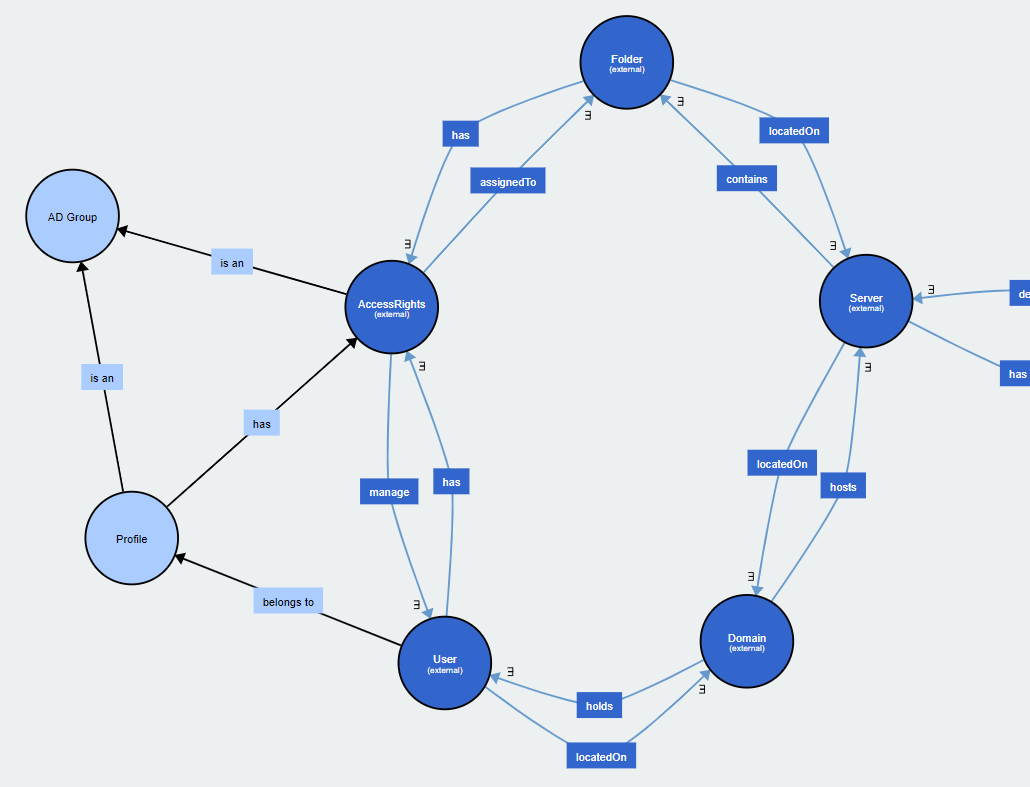
\includegraphics[width=1\textwidth]{Thesis/Images/OntologyProfiles.png}
\end{center}


%%%%%%%%%%%%%%%YIKES

Query String Refinement\newline
Wird nach Testfällen gesucht, in denen ein Schreibrecht gesetzt oder entzogen wird, ist die Ergebnismenge zunächst sehr groß. Durch eine präzisere Suchanfrage ist es möglich, beispielweise zusätzlich zu Schreibrecht noch nach bestimmten Domänenmodi, oder nach UI oder Active Directory (Zugriffsverwaltung von Windows) Tests zu suchen. Durch die Beziehungen in der Ontologie können dann Testfälle, bei denen sich Ordner auf Singledomain Servern befinden und bei denen ein Schreibrecht gesetzt wird als Ergebnis geliefert werden, da zu jedem Ordner ein Server gehört, dem ein bestimmter Domainmode zugewiesen ist.

%%%%%%%%%%%%%%%%%%%YIKES
Inference\newline
Ähnlich wie bei dem Beispiel für "Query String Refinement" gelten für die Testfälle durch das Netz an Beziehungen einige Implikationen, wie der DomainMode, der einem Server zugehörig ist und somit auch einem Ordner. Wird dabei noch berücksichtigt, dass manche DomainModes Fremddomänen nicht zulassen, kann man nur anhand des Ordners bereits einige Rückschlüsse ziehen.\\
%%%%%%%%%%%YIKES

Cross Referencing \newline
Assoziationen lassen sich bei den Testfällen zum Beispiel bei Profiltests und Usertests sehen. Beide Testarten sind Berechtigungsmanagement Tests und betreffen beide das Active Directory. Bei einer Suche nach einem Profiltest können ähnliche Tests aus den Usertests in der Ergebnismenge enthalten sein, da diese z.B. ein sehr ähnliches Verhalten überprüfen und vielleicht sogar voneinander abhängen.\\

Explorative Suche\newline
„Recommended“ Testfälle wirken zunächst ungewöhnlich, könnten aber durchaus einen praktischen Nutzen entwickeln. Wenn ein Verantwortlicher für Produktqualität sich einen Überblick verschaffen möchte, welche Testfälle es bereits gibt, oder welche Features allgemein getestet werden, kann der Verantwortliche durch die Ergebnismenge stöbern, in denen Tests nach Überkategorien sortiert sind, zum Beispiel Profilmanagement und Berechtigungsmanagement, die durch die Implikationen und Assoziationen aus der Ontologie ergeben. Der Verantwortliche für Produktqualität kann so zum Beispiel herausfinden, welche Domainmodes es gibt, wie diese berücksichtigt werden usw., ohne sich ausgiebig mit dem Produkt auseinander zu setzen bevor er die Suche starten kann. Diese Form der Suche entfaltet ihren vollen Nutzen vermutlich bei einer umfassenden Produktabdeckung, also nicht nur kleinen konkreten Testfallbereich, sondern einer Vielzahl an Features und Testfällen, da hier das "stöbern" mehr Kategorien und Inhalt bietet, nach dem sortiert werden kann.

